% !TEX program = xelatex
\documentclass[11pt]{article}
\usepackage{lineno}
\usepackage{amsmath,amssymb,amsthm}
\usepackage{xspace}
\usepackage[margin=3cm]{geometry}
\usepackage[]{todonotes}
\usepackage{mathtools}
%\mathtoolsset{showonlyrefs}
\usepackage{minted}
% requires pygments, e.g. pip install pygments. 
% If you do not install pygments globally on system python, 
% then you might need to add pygmentize to $PATH, 
% e.g. in .zprofile (because this is not an interactive shell), add
%
%	export PATH=$PATH:$(which pygmentize)
%
\setminted[python]{breaklines=true,linenos}
\usemintedstyle{staroffice}
\usepackage{microtype}

\usepackage[hyphens]{url}
\usepackage[colorlinks = true,
    citecolor = blue,
    linkcolor = blue]{hyperref}
\usepackage{fontspec}
\setmonofont[Scale=0.9]{Hasklig}

\newcommand{\dd}{\mathop{}\!\mathrm{d}}
\let\del\partial \newcommand{\dv}[2]{\frac{\dd#1}{\dd#2}} \newcommand{\pdv}[2]{\frac{\partial#1}{\partial#2}} \newcommand{\bangle}[1]{\left\langle#1\right\rangle}
\newcommand{\oldRe}[0]{\Re} \newcommand{\oldIm}[0]{\Im} \let\Re\relax
\let\Im\relax \DeclareMathOperator{\Re}{Re} \DeclareMathOperator{\Im}{Im}

%%%%% widecheck implementation
%%%%%
\usepackage{scalerel,stackengine}
\stackMath
\newcommand\widecheck[1]{%
    \savestack{\tmpbox}{\stretchto{%
            \scaleto{%
                \scalerel*[\widthof{\ensuremath{#1}}]{\kern-.6pt\bigwedge\kern-.6pt}%
                {\rule[-\textheight/2]{1ex}{\textheight}}%WIDTH-LIMITED BIG WEDGE
            }{\textheight}% 
        }{0.5ex}}%
    \stackon[1pt]{#1}{\scalebox{-1}{\tmpbox}}%
}

%%%%%% BB1
%%%%%%https://tex.stackexchange.com/questions/488/blackboard-bold-characters
\DeclareSymbolFont{bbold}{U}{bbold}{m}{n}
\DeclareSymbolFontAlphabet{\mathbbold}{bbold}
\newcommand{\ind}[0]{\mathbbold{1}}

\newcommand{\coloneq}{\mathrel{\mathop:}=}
\newcommand{\eqcolon}{=\mathrel{\mathop:}}

%just a reminder that \lesssim has an opposite \gtrsim

% THEOREMS -------------------------------------------------------
%\newtheorem{thm}{Theorem}
%\newtheorem{cor}[thm]{Corollary}
%\newtheorem{lem}[thm]{Lemma}
%\newtheorem{prop}[thm]{Proposition}
%\theoremstyle{definition}
%\newtheorem{question}[thm]{Question}
%\newtheorem{defn}[thm]{Definition}
%\newtheorem{example}[thm]{Example}
%\theoremstyle{remark}
%\newtheorem{rem}[thm]{Remark}
%\numberwithin{equation}{section}
\usepackage[framemethod=tikz]{mdframed}
\mdfdefinestyle{tao}{linecolor=white,roundcorner=5pt,innertopmargin=0,backgroundcolor=yellow!7!white}
\newmdtheoremenv[style=tao]{theorem}{Theorem}
\newmdtheoremenv[style=tao]{corollary}[theorem]{Corollary}
\newmdtheoremenv[style=tao]{lemma}[theorem]{Lemma}
\newmdtheoremenv[style=tao]{proposition}[theorem]{Proposition}
\newmdtheoremenv[style=tao]{conjecture}[theorem]{Conjecture}
\theoremstyle{definition}
\newmdtheoremenv[style=tao]{definition}[theorem]{Definition}
\newmdtheoremenv[style=tao]{example}[theorem]{Example}
\newmdtheoremenv[style=tao]{exercise}[theorem]{Exercise}
% \theoremstyle{remark}
\newmdtheoremenv[style=tao]{remark}[theorem]{Remark}
\newmdtheoremenv[style=tao]{note}[theorem]{Note}
\newmdtheoremenv[style=tao]{question}[theorem]{Question}

% NAMES ----------------------------------------------------------
\newcommand{\Holder}{H\"older\xspace}

% extras

\DeclareMathOperator{\dil}{dil}
\DeclareMathOperator{\shr}{shr}
\DeclareMathOperator{\rot}{rot}
\DeclareMathOperator{\trans}{tsp}
\DeclareMathOperator{\supp}{supp}


\newcommand{\Var}{\operatorname{Var}}
\newcommand{\E}{\operatorname{\mathbb E}}
\newcommand{\R}{\mathbb R}
\newcommand{\Bias}{\operatorname{Bias}}
\newcommand{\RSS}{\operatorname{RSS}}
\newcommand{\RSE}{\operatorname{RSE}}
\newcommand{\SE}{\operatorname{SE}}
\newcommand{\TSS}{\operatorname{TSS}}
\newcommand{\myhref}[2]{\href{#1}{\texttt{#2}}}


\begin{document}
\title{Notes on and around ISLP}
\author{Calvin Khor}

\date{Last compiled: \today}
\maketitle
\section{Resources}
\begin{enumerate}
	\item The website for the book: \url{https://www.statlearning.com} 
	\item Python Solutions to ISLR: \url{https://github.com/botlnec/islp}
	\item Videos accompanying ISLR: \url{https://www.youtube.com/watch?v=LvySJGj-88U&list=PLoROMvodv4rOzrYsAxzQyHb8n_RWNuS1e}
    \item My errata: \url{https://docs.oracle.com/javase/8/docs/api/java/lang/}
    \item These notes: \url{https://dotty.epfl.ch/3.0.0/api}
\end{enumerate}

\section{Statistical Learning}
\subsection{Definitions and Notation}

 In this book, usually $x_1,\dots,x_n \in \R^p$ denotes training data, and $x_0$ is test (out-sample) data. When its capital letters $X_1,\dots X_n$ its a random variable. The $p$ denotes the number of predictors (i.e. independent variables/features/variables). The model is abstractly

\[ Y=f(X)+\epsilon. \tag{2.1} \]
$Y$ is the response/dependent variable. $\epsilon$ is noise inherent to the model: WLOG $ \E\epsilon=0$,  $\Var\epsilon = 1$, and independent from the predictors (i.e. we cannot predict the error)

We denote the number of observations by $n$, so that the observations of the predictors are $x_j=(x_{1j}, x_{2j},\dots x_{nj})$, for $j=1,\dots,p$.

\subsection{Parametric and non-parametric models}
A parametric model is when the space of solutions can be parameterised by some subset of $\mathbb R^n$. A model is non-parametric otherwise; for instance the model may be parameterised over a subset of functions (e.g. cubic splines.)

\subsection{Prediction Accuracy}

\subsection{Model Interpretability}

\subsection{Test MSE}

Variance: `the amount by which $\hat f$ would change if we estimated it using a different training data set.' - i.e. variance by treating the training data as random variables

Bias: the error that is introduced by approximating a real-life problem, which may be extremely complicated, by a much simpler model. 

\[ E|y_0 - \hat f(x_0)|^2 = \Var\hat f(x_0) + (\Bias \hat f(x_0))^2 + \Var\epsilon \tag{2.7} \]
{\color{red}\fbox{Important quote from book:}}
\begin{quote} Here the notation $\E|y_0 - \hat f(x_0)|^2$ defines the expected test MSE at $x_0$, expected test MSE and refers to the average test MSE that we would obtain if we repeatedly estimated $f$ using a large number of training sets, and tested each at $x_0$. The overall expected test MSE can be computed by averaging $\E|y_0 - \hat f(x_0)|^2$ over all possible values of $x_0$ in the test set. 	
\end{quote}
In other words, the general process is as follows:
\begin{gather*}
\fbox{gather data} \\ x_1,\dots,x_n;\ y_1,\dots,y_n\\ \downarrow \\
\fbox{model choice} \\ Y = f(X) + \epsilon\\ \downarrow \\
\fbox{choose $\hat f$ using data}
\\ \downarrow \\
\fbox{evaluate at out-sample(s)}
\\
\hat y = \hat f(x_0)
\end{gather*}
When we use $\hat f(x_0)$ in discussions of theoretical probability like the above say $\E g(\hat f(x_0), y_0)$, we mean to analyse the above process in the following manner: the expectations are always taken by assuming the data $x_1,\dots,x_n$ are replaced by random variables $X_1,\dots,X_n$. The dependence on these random variables can be written explicitly as $\hat f(x_0) = \hat f(X_1,\dots, X_n; x_0)$, with the test data $(x_0,y_0)$ kept non-random. Then the expected value at a particular test data is
\[ \E g(\hat f(x_0), y_0) = \E_{X_1,\dots,X_n} g(\hat f(X_1,\dots, X_n; x_0), y_0)\]
One can from this model get the `overall expected test MSE' by further averaging over all $(x_0, y_0)$s in some way.

Derivation of (2.7): 
\begin{align*}
\operatorname{LHS}(2.7)
&=  \E|f(x_0) - \hat f(x_0) + \epsilon|^2 \\
&= \E|f(x_0) - \E \hat f(x_0) + (\E \hat f(x_0) - \hat f(x_0)) + \epsilon|^2 \\
&= \E|f(x_0) - \E\hat f(x_0)|^2 + \E|\epsilon|^2 + \E|\hat f(x_0) - \E\hat f(x_0)|^2 + 2\E\epsilon (f(x_0) - \hat f(x_0) ) \\
&= | f(x_0) - \E\hat f(x_0)|^2 + \E|\epsilon|^2 + \E|\hat f(x_0) - \E\hat f(x_0)|^2 + 2\E\epsilon (f(x_0) - \hat f(x_0) ) \\
&=: \Bias^2 + \Var\epsilon + \Var\hat f(x_0) + \underbrace{0}_{ \mathclap{\text{ since }\epsilon\text{ is independent}}} = \operatorname{RHS}(2.7).
\end{align*}

\subsection{Bias-Variance Trade-off}


\section{Linear Regression}
\subsection{Simple Linear Regression}
Model:
\[ Y = \beta_0 + \beta_1 X + \epsilon\]
in particular then \(\E [Y|X]  = \beta_0 + \beta_1 X\). We say "$Y$ regresses on $X$" to indicate that $Y$ is the dependent variable that depends on the independent variable $X$.

Asides: assumptions on $\epsilon$ affects the statistical results one can prove. Ways to work around somewhat: \myhref{https://en.wikipedia.org/wiki/Quasi-maximum_likelihood_estimate}{quasi maximum likelihood} ("departure from Gaussianity". Note Student's $t$ distribution has infinite variance if $nu<2$ and infinite  skewness if $\nu<3$. \myhref{https://en.wikipedia.org/wiki/Kolmogorov–Smirnov_test}{Kolmogorov-Smirnov test}, Kurtosis \url{https://en.wikipedia.org/wiki/Kurtosis}

Prediction = find $\beta_i$ so that 
\[ \hat y := \hat\beta_0 + \hat\beta_1 X\]
minimises the loss. The estimation error at \(x\) is
\[ e \equiv y - \hat y = y - (\hat\beta_0 + \hat\beta_1 x)\]
which may be different from $\epsilon$. OLS = minimising residual sum of squares, \(\RSS = \sum_{i=1}^n e_i^2\). RSS defines your "risk tolerance"; there are different loss functions.


\subsubsection{Estimating the Coefficients}
\[ \hat\beta_1 = \frac{ \sum_i (x_i - \bar x )(y_i - \bar y) }{\sum_i (x_i -\bar x)^2 }\quad (\frac{\text{sample covariance}}{\text{sample variance of $x$}}),\qquad \hat \beta_0 = \bar y - \hat \beta_1 \bar x\]
 
\subsubsection{Assessing the Accuracy of the Coefficient Estimates}
This subsection deals with CE and hypothesis testing to check if there is a (linear) relationship between the data.

The \href{https://en.wikipedia.org/wiki/Standard_error}{\texttt{standard error}} of a statistic (usually an estimate of a parameter) is the standard deviation of its sampling distribution or an estimate of that standard deviation. If the statistic is the sample mean, it is called the standard error of the mean (SEM). The standard error is a key ingredient in producing confidence intervals.

The formula for the (approximate) 95\% CE of $X$ when $X$ is Gaussian is $\hat X \pm 2\SE(\hat X) $. For CEs with different $\alpha$ it would be $\hat X \pm z_{\alpha/2}\SE(\hat X)$. where $z_\theta$ is a Z-statistic.

In the case of the mean
The theorem that the true value lies in the constructed $\alpha$-confidence interval (CE) $\alpha$\% of the time assumes that the error term is Gaussian. Similarly for hypothesis testing.

Hypothesis test if there is a (linear) relationship between $Y$ and $X$: WLOG subtracting the mean, we simply need to test if $\beta_0 = 0$ (the null) or not (the alternative). Accomplished with $t$-statistic  $t=\frac{\hat\beta_1 - 0}{\SE(\hat\beta_1)} \sim t_{n-2}$. Then compute a $p$-value: the probability of getting an observation at least as large as the data, under the null.

There is a correspondence: We reject the null that $\beta_1=0$ iff the confidence interval constructed for $\beta_1$ does not contain 0.

\subsubsection{Assessing the Accuracy of the Model}
After concluding that the model fits the data, we want to quantify how much the model fits.

There is an issue when having too many data points, since the true value of $\beta_0$ is unlikely to be exactly zero in the many observations limit: to avoid this one can use the Akaike Information Criterion, Bayesian Info Criterion: good to use when too many data points so the hypothesis test is statistically significant but not practically significant. Also adjusted $R^2$. "Avoids overfitting".
$\RSE $ is the Residual Standard Error, and $R^2$ is the fraction of variance explained:
\[ \RSE \coloneq \sqrt{\frac{\RSS}{n-2}}, \quad R^2 \coloneq \frac{\TSS - \RSS}{\TSS} = 1 - \frac{\RSS}{\TSS} = 1 - \frac{\sum_{i=1}^n (y_i - \hat y_i)^2}{\sum_{i=1}^n (y_i - \bar y)^2} = 1 - \frac{|y-\hat y|^2}{|y-\bar y \mathbf 1|^2}\]
Note: since OLS is $L^2$ orthogonal projection (after subtracting off the mean),
\[ |y-\bar y \mathbf 1|^2 = |y-\hat y|^2 + |\hat y-\bar y \mathbf 1|^2  \]
In simple linear regression (1 predictor 1 response), $R^2=r^2$ where $r$ is the Pearson correlation coefficient:
\[r = \frac{\sum_{i=1}^n (x_i - \bar x) (y_i - \bar y)}{\sqrt{\sum_{i=1}^n (x_i - \bar x)^2 \sum_{i=1}^n (y_i - \bar y)^2}}.\]
Proof (see Exercise 7, \myhref{https://github.com/botlnec/islp/blob/master/docs/sols/chapter3/exercise7.md}{solution online}): without loss $\bar y=0, \bar x = 0$. Then
\begin{align*}
R^2 
= 1 - \frac{|y-\hat y|^2}{|y|^2}  
= \frac{|\hat y|^2}{|y|^2}  
= \frac{|(X^T X)^{-1} X^T y|^2}{|y|^2} 
\end{align*}
For simple linear regression, $X\in \R^{n\times 1}$ is a column vector so $X^TX = |X|^2$ and $X^Ty = X\cdot y$. Hence 
$R^2 = \left|\frac{X\cdot y}{|X| |y|}\right|^2 = \left|\frac{s_{xy}}{s_x s_y}\right|^2$.
\subsection{Multiple Linear Regression}
Hypothesis testing. $H_0: \beta = (\beta_0,\dots,\beta_n)=0$. $H_1$: there exists one nonzero coefficient. Instead of $t$-statistic, use $F$-statistic.
$y = X\beta + \epsilon$.
Hard to interpret coefficients. Model selection. Dummy variables. Nonlinearities.

\subsection{Other things that came up in class}
\begin{itemize}
    \item \url{https://en.wikipedia.org/wiki/Projection_matrix} (i.e. the hat matrix that puts a hat on $y$, $\hat y = X(X^T X)^{-1} X^T y$.
    \item Random math bit: {\tiny 
Let $f(x) = (1-x^4)^{1/7}$. Observe that on $[0,1]$, $f$ is monotone decreasing with inverse $g(x) = (1-x^7)^{1/4}$. Then if $\mu$ denotes standard Lebesgue measure, we have
\begin{align*}
    \int_0^1 (1-x^4)^{1/7} \dd x &= \int_0^1 f(x) \dd x 
    = \int_0^1 \int_0^{f(x)} \dd t \dd x 
    = \int_0^1 \mu( x\in[0,1] : t<f(x) ) \dd t 
    = \int_0^1 \mu( x\in[0,1] : x<g(t) ) \dd t = \int_0^1 g(t) \dd t \\&= \int_0^1 (1-x^7)^{1/4} \dd x
\end{align*}
PS $d_f(t) \coloneq \mu(x: f(x)>t)$ is the \emph{distribution function} of $f$.}
\item 
Joy's question (difference between interaction features and fitting separate models)
Say we have a problem we're modelling as $y=X\beta + \epsilon\quad (\in\mathbb R)$. 
We can then e.g. choose to double the number features by elementwise multiplying by appropriate indicators: i.e. if $X^C= X \texttt{*.}\mathbf 1_C$ for some condition $C$ (forgive my abuse $(\mathbf 1_C)_i \coloneq \mathbf 1_{i\in C}$ for $i=1,\dots,n$)  then $X=X^C + X^{C^c}$.
    To fix notation, WLOG set $C = [1,c]$, 
    $X^C = \binom{A}{0}$ and $X^{C^c}= \binom{0}{B}$ 
    where $A\in \mathbb R^{c\times p}$ 
    and $B\in \mathbb R^{d\times p}$, $c+d=n$  
    (so that $\tilde X = \text{\tiny $\begin{pmatrix} A & 0 \\ 0 & B \end{pmatrix}$}\in \mathbb R^{(c+d)\times 2p}$ 
    is the new features matrix). Then the $2p$ predictors model can be written 
    \[ \binom{y^1}{y^2} = y = \tilde X \tilde \beta + \epsilon = A\beta^1 + B\beta^2 + \epsilon.\]
    OLS will find the unique $\tilde \beta=\binom{\beta^1}{\beta^{2}}$ that minimises
    \begin{align}
        \sum_{i=1}^{n} \left|y_i -  \sum_{j=1}^{2p}\tilde X_{ij} \tilde \beta_j \right|^2 
        &= \sum_{i\in C} \left|y_i -  \sum_{j=1}^{2p}\tilde X_{ij} \tilde \beta_j \right|^2  + \sum_{i\not\in C} \left|y_i -  \sum_{j=1}^{2p}\tilde X_{ij} \tilde \beta_j \right|^2 \\
        &= \sum_{i\in C} \left|y_i -  \sum_{j=1}^{p} X^C_{ij}  \beta^1_j \right|^2  + \sum_{i\not\in C} \left|y_i -  \sum_{j=1}^{p} X_{ij}^{C^c} \beta^2_j \right|^2.
    \end{align}
    Since $\beta^i$ are independently chosen this solution is (uniquely) given by the minimisers of each of the two summands. We can also relate this to smaller models that are fit separately on the $i\in C$ and $i\not\in C$ data:
        \begin{align}
        \sum_{i=1}^{n} \left|y_i -  \sum_{j=1}^{2p}\tilde X_{ij} \tilde \beta_j \right|^2 
        &= \sum_{i=1}^c \left|y_i^1 -  \sum_{j=1}^{p} A_{ij} \beta_j^1 \right|^2 + \sum_{i=1}^d \left|y_i^2 -  \sum_{j=1}^{p} B_{ij} \beta_j^2 \right|^2.
        \end{align}
    One can plainly read off the two summands as the loss functions for the separate models. And just for completeness, the OLS solution for the $2p$ predictor model is 
    \begin{align}
      \hat{\tilde \beta} &=   (\tilde X^T \tilde X)^{-1} \tilde X^Ty \\
      &= \begin{pmatrix}
          (A^TA)^{-1} & 0 \\ 
          0 & (B^TB)^{-1}
      \end{pmatrix}
      \begin{pmatrix}
          A^T & 0 \\ 0 & B^T 
      \end{pmatrix} \binom{y^1}{y^2} = \binom{(A^TA)^{-1} A^T y^1 }{(B^T B)^{-1} B^T y^2}.
    \end{align}
\end{itemize}

    
\section{Classification}
\subsection{Overview}
\subsection{Why not Linear Regression}
\subsection{Logistic Regression}
\subsubsection{Multiple Logistic Regression}
\subsubsection{Multinomial Logistic Regression}
\subsection{Generative Models for CLassification}
\subsubsection{Linear Discriminant Analysis}
\subsubsection{Quadratic Discriminant Analysis}
\subsubsection{Naive Bayes}
\subsection{Comparison to $K$NN}
\subsection{Generalised Linear Models}

\section{}
\section{}
\section{}
\section{Tree-based Methods}
\section{}
\section{}
\section{Quick notes on using scikit-learn and Pandas}
\subsection{Introduction}
While I was trying to learn these tools for data analysis, I found the available discussion online to be dated. These notes aim to get you using the newer features of scikit-learn quickly, to the point where you are comfortable creating your own estimators.
\subsubsection{Setup}
I will assume semi-recent versions of python (3.11), numpy (1.26), scipy (1.11.x), scikit-learn (1.3.2) and so on.

In the first block of your Jupyter notebook I would keep all the imports that you add later, so that it is easy to restart. I would also recommend settings like the following:
\begin{minted}{python}
import pandas as pd
pd.options.display.max_columns = 1000
pd.options.display.max_rows = 2000
pd.options.display.width = 1000
pd.options.display.max_colwidth = 400
\end{minted}
Since \myhref{https://scikit-learn.org/stable/auto_examples/release_highlights/plot_release_highlights_1_2_0.html}{scikit-learn 1.2}, there is good interop with Pandas: you can configure all transformers to output pandas DataFrames globally.
\begin{minted}{python}
from sklearn import set_config
set_config(transform_output="pandas")
\end{minted}

\subsection{Basic Usage}
We will assume that we are trying to perform prediction on some labelled training data which we will store in \mintinline{python}!X!, \mintinline{python}!y!, and the test data in \mintinline{python}!X_test!.
\begin{minted}{python}
X = pd.read_csv("X_train.csv") 
y_raw = pd.read_csv("Y_train.csv")  
X_test = pd.read_csv("X_test.csv")
y = y_raw["TARGET"]
\end{minted}

We will first assume that we want to design a \mintinline{python}!Pipeline!, fit it to the training data, predict with a regressor, and try to evaluate our performance. Later, we will see how to modify this to allow for gridsearching.

\subsubsection{Pipeline}
A a \mintinline{python}!Pipeline! is a way to combine estimators and predictors in a way that is easy to modify and develop. Documentation on \mintinline{python}!Pipeline!s \myhref{https://scikit-learn.org/stable/modules/compose.html\#build-a-pipeline}{here}. To understand them, we have to first explain what scikit-learn estimators are: these are the building blocks that either transform your data, or learn and predict from them. 
An estimator \mintinline{python}!MyEstimator! is implemented as a Python class (usually inheriting from \mintinline{python}!BaseEstimator!). 
If it transforms, it has an \mintinline{python}!MyEstimator.transform! method;
learning is done with the \mintinline{python}!MyEstimator.fit! method, and
prediction is done with the \mintinline{python}!MyEstimator.predict! method. 

An example of a transformer is \mintinline{python}!StandardScaler! which\footnote{another useful scaler is the \mintinline{python}!RobustScaler! which uses quantile information and is therefore more robust to outliers.} scales to mean 0 and variance 1. 
One needs to fit to learn the parameters and then transform, or the convenience method \mintinline{python}!fit_transform!:
\begin{minted}{python}
from sklearn.preprocessing import StandardScaler
X_scaled = StandardScaler().fit(X).transform(X) 
X_scaled = StandardScaler().fit_transform(X) # same as the above
\end{minted}
A very convenient transformer is the \mintinline{python}!FunctionTransformer! which applies an arbitrary Python function to the Pandas \mintinline{python}!DataFrame!. The function should take the dataframe as input, and return a new dataframe, which is the output of the \mintinline{python}!transform! method (\mintinline{python}!fit! is empty for \mintinline{python}!FunctionTransformer!s.) A simple example is if you wanted to drop a column called \mintinline{python}!"Rubbish"!, you could use\footnote{Keep in mind though lambdas will prevent the transformer from pickling.}
\begin{minted}{python}
from sklearn.preprocessing import FunctionTransformer
X_clean = FunctionTransformer(lambda df: df.drop(["Rubbish"], axis=1)).transform(X)
\end{minted}

Once we are happy with the preprocessing, we need to make the predictions. For example we can fit e.g.\footnote{This includes the intercept term by default.} \mintinline{python}!LinearRegression! and predict on the test data:
\begin{minted}{python}
    from sklearn.linear_model import LinearRegression
    ols = LinearRegression().fit(X,y)
    y_test = ols.predict(X_test)
\end{minted}
The last thing to do is to evaluate the performance of our model. This will be project specific. The short answer is to use cross-validation since it is a model agnostic method of estimating the true error on an unforseen dataset, which is good for iterating to more complicated models. Cross-validation is implemented as part of many different functions in \texttt{scikit-learn} but for starters one can \mintinline{python}!from sklearn.model_selection import cross_validate!. 

One can also use the training error as a rough upper bound but don't get too attached to it. Since we have the target predictions on the training set, we can plot the data. Below, I have some convenience functions defined in order to quickly evaluate the cross-validation score and plot the model's predictions against the target predictions. I'm using Spearman's rank correlation coefficient as a scoring method, which works better for nonlinear data.

\begin{minted}{python}
from scipy.stats import spearmanr
from sklearn.metrics import make_scorer
from sklearn.preprocessing import QuantileTransformer
import matplotlib.pyplot as plt
import seaborn as sns


def spearman_metric(y_pred, y=y):
    """y_pred is the model prediction; y is the training data target"""
    return spearmanr(y_pred, y).correlation
spearman_scorer = make_scorer(spearman_metric)


def grade(y_pred, y=y) -> None:
    Xy = X[["COUNTRY"]].copy()
    Xy["TARGET"] = y
    Xy["PREDICTED"] = y_pred
    Xy[["TARGET", "PREDICTED"]] = QuantileTransformer().fit_transform(
        Xy[["TARGET", "PREDICTED"]]
    )

    _, ax = plt.subplots()
    plt.plot(Xy["TARGET"], Xy["TARGET"], label="y=x (perfect model)", alpha=0.3)
    sns.scatterplot(Xy, y="PREDICTED", x="TARGET", hue="COUNTRY", alpha=0.8, s=20)
    plt.xlabel("Actual Values" + (" (quantile)" if quantile else ""))
    plt.ylabel("Predicted Values" + (" (quantile)" if quantile else ""))
    plt.title(
        "Output vs Training Data\nSpearman correlation for the train set: {:.1f}%".format(
            100 * spearman_metric(y_pred, y)
        )
    )
    ax.legend(title=None)
    plt.show()


def perform_cv(
    estimator, data, cv=5, scorer=spearman_scorer, show=True, y=y, n_jobs=1, verbose=0
) -> pd.DataFrame:
    """displays cv test scores and returns the result from the cv.
    """
    cv_results = cross_validate(
        estimator, data, y, cv=cv, scoring=scorer, n_jobs=n_jobs, verbose=verbose
    )
    if show:
        # Print the mean and standard deviation of the test scores
        print(
            "Spearman correlation for the cross validation: {:.1f}% ± {:.1f}%".format(
                100 * cv_results["test_score"].mean(),
                100 * cv_results["test_score"].std(),
            )
        )
        print(f"Spearman correlation for each fold: {cv_results['test_score']}")
    return pd.DataFrame(cv_results)
\end{minted}
\subsubsection{Finally, the Pipeline}
The upshot of the above code is that Pipelines allow me to perform the entire data analysis in a very short Jupyter code block:
\begin{minted}{python}
pipe = Pipeline(
    [
        ("drop", FunctionTransformer(lambda df: df.drop(["COUNTRY"], axis=1))),
        ("scale", RobustScaler()),
        ("ols", LinearRegression()),
    ]
)
pipe.fit(X, y)
y_pred = pipe.predict(X)
grade(y_pred, y)
perform_cv(pipe, X)
\end{minted}
What a Pipeline is then, is a way to convert a sequence of transformers and a final predictor into a single estimator. 
Calling \mintinline{python}!pipe.fit(X,y)! is equivalent to calling \mintinline{python}!fit_transform! on every transformer and fit on the predictor; calling \mintinline{python}!pipe.predict! calls \mintinline{python}!transform! on all the transformers and then \mintinline{python}!predict!:
\begin{minted}{python}
# need to define the estimators separately if not using a pipeline
drop = FunctionTransformer(lambda df: df.drop(["COUNTRY"], axis=1))
scale = RobustScaler()
ols =  LinearRegression()
# below is the same as pipe.fit(X,y)
ols.fit(scale.fit_transform(drop.fit_transform(X)),y) 
# below is the same as y_pred = pipe.predict(X)
y_pred = ols.predict(scale.transform(drop.transform(X))) 
\end{minted}
Note in particular that the order of appearance of each estimator in the pipeline corresponds to the order in which they are called, but it is reversed (and nested) in the non-pipeline version.

To use a pipeline, simply pass a list of tuples to the constructor. The second part of the tuple is simply the estimator, and the first part\footnote{There is a variant, \mintinline{python}!make_pipeline! that avoids needing a name by creating a default one from the transformer.
} is a name that can be used to inspect parts of the pipe:
\begin{minted}{python}
# this pulls out the coefficients computed from ols
pipe_bench.named_steps["ols"].coef_
\end{minted}
\subsection{Gridsearching}
Suppose instead of \mintinline{python}!LinearRegression!, we wanted to use \mintinline{python}!Lasso!, which modifies the loss function for least squares by an \(L^1\) penalty term for the coefficients, i.e.
\[ J(\beta) = \sum_{i=1}^n\lvert y_i-(X\beta)_i\rvert^2 + \alpha \sum_{j=1}^p\lvert\beta_j\rvert\]
The parameter \(\alpha\) can be interpreted as a Lagrange multiplier. But since this minimisation problem cannot be solved symbolically, we have to treat it as a \emph{tuning parameter} and determine it experimentally.

To use lasso, we import it and set up our pipeline:
\begin{minted}{python}
from sklearn.linear_model import Lasso
pipe = Pipeline(
    [
        ("drop", FunctionTransformer(lambda df: df.drop(["COUNTRY"], axis=1))),
        ("scale", RobustScaler()),
        ("lasso", Lasso()),
    ]
)
\end{minted}
\texttt{scikit-learn} has many ways to search for an optimal parameter. The simplest is \mintinline{python}!GridSearchCV!, which performs an exhaustive search in the given parameter space. I have written some helper functions (\mintinline{python}!display_grid_params! and \mintinline{python}!report!) as well.
The overall code is as follows:
\begin{minted}{python}
from icecream import ic
import time
# pipe code from above goes here
tick = time.time()
pipe.fit(X, y)
time_for_one_fit = time.time() - tick
ic(time_for_one_fit)
param_grid = {
    "model__alpha": [ 0.2 * np.exp(0.01 * k) for k in range(-5, 5)],
}
display_grid_params(param_grid, time_for_one_fit)
grid = GridSearchCV(
    pipe, param_grid=param_grid, cv=5, n_jobs=-1, scoring=spearman_scorer
)
grid.fit(X, y)
report(grid)
print("Predicting on train set using best params above:")
y_best = grid.predict(X)
grade(y_best, y)
\end{minted}
For completeness, the helper functions are:
\begin{minted}{python}
from icecream import ic
import functools
from operator import mul 
def display_grid_params(params, time_for_one_fit=None):
    params_size = functools.reduce(mul, (len(params[k]) for k in params))
    note = f"The params grid has size {params_size}. "
    if time_for_one_fit:
        min, sec = divmod(time_for_one_fit * params_size, 60)
        hr, min = divmod(min, 60)
        note += f"Estimated time to completion: {hr}h {min}m {sec:.1f}s"
    ic(note)
    ic(params)


def report(grid, n_top=3):
    """Usage: fit outside the report with grid.fit(X,y). Then pass the cv_results_ to report.
    """
    cv_results_ = grid.cv_results_
    grid_df = pd.DataFrame(cv_results_)[
        ["params", "mean_test_score", "std_test_score", "rank_test_score"]
    ].sort_values(by="rank_test_score")

    if n_top != 0:
        ic(grid.best_params_, grid.best_score_)
    if n_top > 0:
        display(grid_df.head(n_top))
    elif n_top < 0:
        display(grid_df)
    return grid_df
\end{minted}
See \myhref{https://scikit-learn.org/stable/modules/grid_search.html}{this part} of the User Guide for more complicated (and potentially more efficient) methods of tuning hyper-parameters.
\subsection{The need for custom estimators}
The built-in estimators are powerful: 
you can \myhref{https://scikit-learn.org/stable/auto_examples/preprocessing/plot_all_scaling.html\#plot-all-scaling-robust-scaler-section}
{scale},
\myhref{https://scikit-learn.org/stable/modules/impute.html\#impute}
{impute missing values},
\myhref{https://scikit-learn.org/stable/modules/feature_selection.html\#feature-selection}
{select features},
\myhref{https://scikit-learn.org/stable/modules/ensemble.html}
{combine predictors together}, 
and so on (see the 
\myhref{https://scikit-learn.org/stable/user_guide.html}
{User Guide}.) 
But there are times when one has an idea that is hard to express with the defaults. 
For this one needs to know how to create a custom estimator. See scikit-learn's 
\myhref{https://scikit-learn.org/stable/developers/develop.html}
{own tutorial}.
We can start from the following useful but simple example, which I call
\mintinline{python}!Tap!:
\begin{minted}{python}
class Tap(BaseEstimator, TransformerMixin):
    """debugger"""

    def __init__(self) -> None:
        pass

    def fit(self, X: pd.DataFrame, y=None):
        self.X_ = X.copy()
        return self

    def transform(self, X):
        return X
\end{minted}
Essentially, we always inherit from \mintinline{python}!BaseEstimator!
(\myhref{https://scikit-learn.org/stable/modules/generated/sklearn.base.BaseEstimator.html\#sklearn.base.BaseEstimator.get_params}
{which} defines \mintinline{python}!.get_params! and \mintinline{python}!.set_params!). 
Adding the \mintinline{python}!TransformerMixin! defines\footnote{
it also defines \myhref{https://scikit-learn.org/stable/modules/generated/sklearn.base.TransformerMixin.html\#sklearn-base-transformermixin}
{set\_output} for Pandas, but the global setting is enough.
} \mintinline{python}!fit_transform!, given that \mintinline{python}!fit! and \mintinline{python}!transform! are defined. 

The only point of this class is so to save the DataFrame passed to it so that it can be inspected later. This helps with the development of other estimators and understanding your model.

\mintinline{python}!Tap! doesn't need any parameters so the initialiser is empty. For more complicated estimators, I first quote from scikit-learn's \myhref{https://scikit-learn.org/stable/developers/develop.html}
{own tutorial} an important point for interop with the scikit-learn estimators:
\begin{quote}
The object’s \mintinline{python}!__init__! method might accept constants as arguments that determine the estimator’s behavior (like the C constant in SVMs). It should not, however, take the actual training data as an argument, as this is left to the \mintinline{python}!fit()! method:
\begin{minted}{python}
clf2 = SVC(C=2.3)
clf3 = SVC([[1, 2], [2, 3]], [-1, 1]) # WRONG!
\end{minted}
The arguments accepted by \mintinline{python}!__init__! should all be keyword arguments with a default value. In other words, a user should be able to instantiate an estimator without passing any arguments to it. The arguments should all correspond to hyperparameters describing the model or the optimisation problem the estimator tries to solve. These initial arguments (or parameters) are always remembered by the estimator. Also note that they should not be documented under the “Attributes” section, but rather under the “Parameters” section for that estimator.

In addition, every keyword argument accepted by \mintinline{python}!__init__! should correspond to an attribute on the instance. Scikit-learn relies on this to find the relevant attributes to set on an estimator when doing model selection.

To summarize, an \mintinline{python}!__init__! should look like:
\begin{minted}{python}
def __init__(self, param1=1, param2=2):
    self.param1 = param1
    self.param2 = param2
\end{minted}
There should be no logic, not even input validation, and the parameters should not be changed. The corresponding logic should be put where the parameters are used, typically in fit. 

[\dots]

The reason for postponing the validation is that the same validation would have to be performed in \mintinline{python}!set_params!, which is used in algorithms like \mintinline{python}!GridSearchCV!.
\end{quote}
Notably, the above convention is at odds with the usual Python conventions. With that out of the way, I present my \mintinline{python}!ColumnSubset! meta-estimator, which allows you to specify a column name, a list of names, or a function that transforms \mintinline{python}!X.columns! into the required list of column names, and then apply a transformer only to those columns. This \emph{can} be done in the simpler cases with \href{https://scikit-learn.org/stable/modules/generated/sklearn.pipeline.FeatureUnion.html}{\mintinline{python}!FeatureUnion!} or \href{https://scikit-learn.org/stable/modules/generated/sklearn.compose.ColumnTransformer.html\#sklearn-compose-columntransformer}{\mintinline{python}!ColumnTransformer!} which come with \texttt{scikit-learn}, but I didn't like how \mintinline{python}!ColumnTransformer! changed the names of my columns, and I wanted more flexibility in choosing the columns.
\begin{minted}{python}
Estimator = Pipeline # just for type hinting
def column_subset(
    X: pd.DataFrame,
    columns: str | list[str] | Callable | None = None,
    ignore_columns: str | list[str] | Callable | None = None,
):
    if isinstance(columns, str):
        out = [columns]
    elif isinstance(columns, list):
        out = columns
    elif callable(columns):
        out = columns(X.columns)
    elif columns is None:
        out = X.columns
    else:
        raise TypeError(f"Invalid type for columns={columns}")

    if isinstance(ignore_columns, str):
        out = [c for c in out if c != ignore_columns]
    elif isinstance(ignore_columns, list):
        out = [c for c in out if c not in ignore_columns]
    elif callable(ignore_columns):
        out = [c for c in out if c not in ignore_columns(X.columns)]
    elif ignore_columns is None:
        pass
    else:
        raise TypeError(f"Invalid type for ignore_columns={ignore_columns}")

    return (out, [c for c in X.columns if c not in out])


class ColumnSubset(BaseEstimator, TransformerMixin):
    def __init__(
        self,
        estimator: Estimator,
        columns: str | list[str] | Callable | None = None,
        ignore_columns: str | list[str] | Callable | None = None,
    ) -> None:
        self.estimator = estimator
        self.columns = columns
        self.ignore_columns = ignore_columns

    def fit(self, X: pd.DataFrame, y=None):
        self.cols_, self.other_cols_ = column_subset(
            X, columns=self.columns, ignore_columns=self.ignore_columns
        )
        self.estimator.fit(X[self.cols_], y)
        return self

    def transform(self, X: pd.DataFrame):
        return pd.merge(
            X[self.other_cols_],
            self.estimator.transform(X[self.cols_]),
            left_index=True,
            right_index=True,
\end{minted}
I also created \mintinline{python}!ModelTransformer!, for using an (unsupervised) model's predictions to transform my features:
\begin{minted}{python}
class ModelTransformer(BaseEstimator, TransformerMixin):
    """The `ModelTransformer` class is a custom transformer that fits a model on specified independent and
    response columns, and transforms the input data by predicting the response values using the fitted
    model."""

    def __init__(
        self,
        model: Estimator,
        indep_cols: list[str],
        response_cols: list[str],
    ):
        self.model = model
        self.indep_cols = indep_cols
        self.response_cols = response_cols

    def fit(self, X, y=None):
        self.model.fit(X[self.indep_cols], X[self.response_cols])
        return self

    def transform(self, X: pd.DataFrame):
        pre_out = pd.DataFrame(
            self.model.predict(X[self.indep_cols]),
            columns=[f"MT_{c}" for c in self.response_cols],
            index=X.index,
        )

        return = pd.merge(
            X,
            pre_out,
            left_index=True,
            right_index=True,
        )
\end{minted}

Finally, I want to share my \mintinline{python}!ModelSelector!, which switches between predictors based on a categorical variable. This allows you to fit two (or inductively, any number) different models in a single Pipeline.
\begin{minted}{python}
class ModelSelector(BaseEstimator, RegressorMixin):
def __init__(
    self,
    model_0: Estimator,
    model_1: Estimator,
    cat_var: str,
    drop_cat_var: bool = False,
):
    self.model_0 = model_0  
    self.model_1 = model_1 
    self.cat_var = cat_var
    self.drop_cat_var = drop_cat_var

def fit(self, X: pd.DataFrame, y):
    # split the data based on the value of the categorical variable
    X_0 = X[X[self.cat_var] == 0]
    y_0 = y[X[self.cat_var] == 0]
    X_1 = X[X[self.cat_var] == 1]
    y_1 = y[X[self.cat_var] == 1]
    if self.drop_cat_var:
        X_0 = X_0.drop(columns=[self.cat_var])
        X_1 = X_1.drop(columns=[self.cat_var])
    # fit the models on the corresponding subsets of data
    self.model_0.fit(X_0, y_0)
    self.model_1.fit(X_1, y_1)
    return self

def predict(self, X):
    # split the data based on the value of the categorical variable
    X_0 = X[X[self.cat_var] == 0]
    X_1 = X[X[self.cat_var] == 1]
    if self.drop_cat_var:
        X_0 = X_0.drop(columns=[self.cat_var])
        X_1 = X_1.drop(columns=[self.cat_var])
    # predict using the models on the corresponding subsets of data
    y_pred_0 = self.model_0.predict(X_0)
    y_pred_1 = self.model_1.predict(X_1)
    # combine the predictions into a single array
    y_pred = np.empty(len(X))
    y_pred[X[self.cat_var] == 0] = y_pred_0
    y_pred[X[self.cat_var] == 1] = y_pred_1
    return y_pred
\end{minted}
\subsection{Further reading}
I have made other more complicated estimators but they are too specific to the dataset. Hopefully the above examples have helped you learn how to use \texttt{scikit-learn} effectively. There are many \myhref{https://scikit-learn.org/stable/auto_examples/index.html}{more examples} on the website and the \myhref{https://scikit-learn.org/stable/user_guide.html}{User Guide} and the \myhref{https://scikit-learn.org/stable/modules/classes.html}{API docs} are very helpful. \section{Python}
% \subsection{Classes}
% https://stackoverflow.com/questions/100003/what-are-metaclasses-in-python

\subsection{Conventions and patterns}
\begin{itemize}
\item Subscript at the end of a variable name means we are looking at a coefficient or other computed quantity of an estimator.	
\item Further to the above, see how to make custom estimators on conventions in the init and other functions (they differ from usual Python classes
\item Don't use \texttt{inplace=True}.
\item Saving a model using Joblib:
\begin{minted}{python}
import joblib
# saving; the filetype extension is only for the user/reader
joblib.dump(pipe, 'filename.joblib') 

# loading
loaded = joblib.load('filename.joblib')
\end{minted}
Make sure you use the same environment (module version etc.) or the model may change.
\item Pipelines are DataFrame-friendly\footnote{This and the next bullet point is from \url{https://www.youtube.com/watch?v=BFaadIqWlAg&list=PLzERW_Obpmv_t55kNFRet-E0h1nKeswWF&index=26}, with Github repo at \url{https://github.com/jem1031/pandas-pipelines-custom-transformers}.}, if the component transformers are as well. If they are not, we can wrap the transformer so that it returns a DataFrame. For instance, \mintinline{python}!StandardScaler! which normally returns a \mintinline{python}!np.array!:
\begin{minted}{python}
class DFStandardScaler(TransformerMixin):
    def __init__(self):
        self.ss = None
    def fit(self, X, y=None):
        self.ss = StandardScaler().fit(X)
        return self    
    def transform(self, X):
        Xss = self.ss.transform(X)
        Xscaled = pd.DataFrame(Xss, index=X.index, columns=X.columns)
        return Xscaled
\end{minted}
\item Pipelines compose\footnote{see also \url{http://zacstewart.com/2014/08/05/pipelines-of-featureunions-of-pipelines.html}}, e.g.:
\begin{minted}{python}
pipeline = Pipeline([
    ('features', DFFeatureUnion([
        ('categoricals', Pipeline([
            ('extract', ColumnExtractor(CAT_FEATS)),
            ('dummy', DummyTransformer())
        ])),
        ('numerics', Pipeline([
            ('extract', ColumnExtractor(NUM_FEATS)),
            ('zero_fill', ZeroFillTransformer()),
            ('log', Log1pTransformer())
        ]))
    ])),
    ('scale', DFStandardScaler())
])    
\end{minted}

\end{itemize}


\subsection{Custom Scikit-learn classes} From \url{https://www.youtube.com/watch?v=WGirN6zBJ4s&list=PLzERW_Obpmv_t55kNFRet-E0h1nKeswWF&index=1}. There are \mintinline{python}!Estimator!, \mintinline{python}!Predictor!, \mintinline{python}!Transformer!, and \mintinline{python}!Model! classes. An \mintinline{python}!Estimator! must implement 
\begin{itemize}
	\item \mintinline{python}!.fit(X,y)!, fitting the estimator to \mintinline{python}!X! and \mintinline{python}!y!
	\item \mintinline{python}!.get_params()! return the parameters of the estimator
	\item \mintinline{python}!.set_params(**params)! change the parameters of the estimator (e.g. for copying)
\end{itemize}
Sklearn's \mintinline{python}!Predictor! needs 
\begin{itemize}
	\item \mintinline{python}!.predict(X)!
\end{itemize}
Sklearn's \mintinline{python}!Transformer! needs 
\begin{itemize}
	\item \mintinline{python}!.transform(X, y=None)!
\end{itemize}
Sklearn's \mintinline{python}!Model! needs 
\begin{itemize}
	\item \mintinline{python}!.score(X,y)!
\end{itemize}
\subsubsection{Inheritance and Mixins}
\begin{itemize}
	\item You can implement \mintinline{python}!.get_params()! and \mintinline{python}!.set_params()! by inheriting from \mintinline{python}!BaseEstimator!
	\item There is also \mintinline{python}!base.TransformerMixin!, \mintinline{python}!base.RegressorMixin!, \mintinline{python}!base.ClassifierMixin!,  \mintinline{python}!base.ClusterMixin!,  \mintinline{python}!feature_selection.SelectorMixin!,\dots
\end{itemize}
\subsubsection{Example 1: Scaler}
\begin{minted}{python}
import numpy as np
from sklearn.base import BaseEstimator, TransformerMixin

class Standardizer(BaseEstimator, TransformerMixin):

def __init__(self,mean_after_transform = 0):
    self.mean_after_transform = mean_after_transform
    
def fit(self, X, y=None):
    self.mean_ = np.mean(X, axis=0) # columwise mean
    self.std_ = np.std(X, axis=0) # columwise std
    return self
    
def transform(self, X):
    return (X-self.mean_) / self.std_ + self.mean_after_transform
\end{minted}
\subsubsection{Example 2: Regression}
Basic regressor that just predicts using the mean or median, using  \mintinline{python}!RegressorMixin! (A regressor is a type of \mintinline{python}{Model}, so it needs a predict. The mixin gives us a \mintinline{python}!.score! for free):
\begin{minted}{python}
import numpy as np
class MyDummyRegression(BaseEstimator, RegressorMixin):

def __init__(self, use_median=False):
    self.use_median = use_median
    
def fit(self, X, y):
    if self.use_median:
        self.value_ = np.median(y)
    else:
        self.value_ = np.mean(y)
    return self
    
def predict(self, X):
    out = np.empty (len(X))
    out.fill(self.value_)
    return out
\end{minted}

\subsection{FeatureUnion, FunctionTransformer, ColumnTransformer}
ColumnTransformer video: \url{https://www.youtube.com/watch?v=to2mukSyvLk&list=PLzERW_Obpmv_t55kNFRet-E0h1nKeswWF&index=22}

\subsection{Keep the index when defining transform}
Example:

\subsection{Don't assign multiple times: concat instead}
This holds for \mintinline{python}!df.assign(key=col)!, \mintinline{python}!df1.merge(df2)!, and \mintinline{python}!df[key]=col!. 

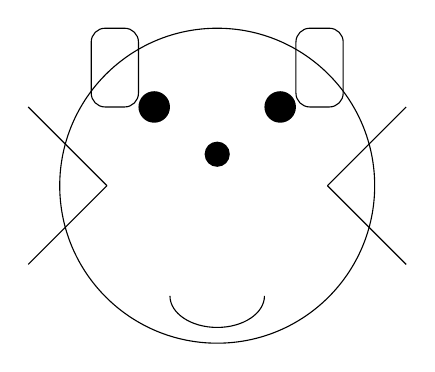
\begin{tikzpicture}[scale=2]
% Head
\draw (0,0) circle (1);
% Eyes
\fill[white] (0.4,0.5) circle (0.15);
\fill[black] (0.4,0.5) circle (0.1);
\fill[white] (-0.4,0.5) circle (0.15);
\fill[black] (-0.4,0.5) circle (0.1);
% Nose
\fill[black] (0,0.2) circle (0.08);
% Mouth
\draw (-0.3,-0.7) arc (180:360:0.3 and 0.2);
% Ears
\draw[rounded corners=5pt] (-0.8,0.5) rectangle (-0.5,1);
\draw[rounded corners=5pt] (0.8,0.5) rectangle (0.5,1);
% Whiskers
\draw (-0.7,0) -- (-1.2,0.5);
\draw (-0.7,0) -- (-1.2,-0.5);
\draw (0.7,0) -- (1.2,0.5);
\draw (0.7,0) -- (1.2,-0.5);
\end{tikzpicture}

\end{document}
